%===================================================================================================
% 実験
%===================================================================================================
\chapter{実験}
本章では,設計したシステムを用いて2種の実験を行う.
1つ目は,音声による水の取り寄せ指示と,それに対するサービスロボットの応答の観測である.
「読書する」,「食事する」,「木を注視する」の3つの異なる行動の最中に,共通の曖昧な音声指示を与え,サービスロボットが適切に応答することを示す.
2つ目は,ユーザの特定の行動に対するサービスロボットの呼びかけである.
明示的な音声指示が与えられる前に,「ロボットを注視する」,「辺りを見回す」の2つの行動を検出して,サービスロボットから能動的に呼びかける.
両方の実験から,1人称視点映像による行動情報がユーザの指示や意図の正確な理解に有効であることを示す.

%---------------------------------------------------------------------------------------------------
\section{実験内容}
\subsection*{水の取り寄せ指示}
表{\ref{tb:experiment_2_1}}に,ユーザから与える音声指示と,行動毎のサービスロボットの応答内容を示す.
また,TMSで管理する物品の中で,水の取り寄せに対して候補となるものを表{\ref{tb:experiment_2_object_list}}に示す.
本研究では,サービス指示に焦点を当て,実際の取り寄せサービスを行わない.
また,サービスロボットが提示する物品名は,TMSデータベースに登録されたものを使用する.
実験手順は次の通りである.
%
\begin{enumerate}
\item{知能化空間内で対象の行動を行う}
\item{行動が認識された時点で水を取り寄せる旨の音声指示を与える}
\item{指示に対してサービスロボットが提示する物品名を確認する}
\end{enumerate}
%
\begin{table}[htbp]
  \begin{center}
  \caption{水の取り寄せ指示と所望の応答}
  \label{tb:experiment_2_1}
    \begin{tabular}{cccl} \bhline{1.2pt}
      音声指示 & 行動 & 適当な物品 & サービスロボットの応答 \\ \hline
      \multirow{3}{*}{Bring me some water.}
      & 読書する & コーヒー & Would you like a cup of coffee ? \\
      & 食事する & お茶 & Would you need a bottle of tea ? \\
      & 植木を注視する & ジョーロ & Would you need a watering pot ? \\ \bhline{1.2pt}
    \end{tabular}
  \end{center}
\end{table}
%
\begin{table}[htbp]
  \begin{center}
  \caption{TMSデータベース内の水に関連する物品}
  \label{tb:experiment_2_object_list}
    \begin{tabular}{cccc} \bhline{1.2pt}
      物品カテゴリ & ID & 物品名 & タグ\\ \hline
      お茶 & 7004 & greentea\_bottle & drink, tea, water \\
      お茶 & 7005 & soukentea\_bottle & drink, tea, water \\
      缶コーヒー & 7006 & cancoffee & drink, coffee, water \\
      ジョーロ & 7026 & watering\_pot & pot, water \\ \bhline{1.2pt}
    \end{tabular}
  \end{center}
\end{table}

\subsection*{特定の行動をトリガとしたサービス}
表{\ref{tb:experiment_2_2}}に,検出対象の行動と,それに対するサービスロボットの応答を示す.ここでは,ユーザがサービスロボットを注視している場合,何かサービスを要求しようとしているものとし,辺りを見回している場合,何かを探しているものと仮定した.すなわち,ユーザの心理的要因による1人称視点の変化をトリガとしたサービスの開始を図る.
実験手順は次の通りである.
%
\begin{enumerate}
\item{知能化空間内で対象の行動を行う}
\item{サービスロボットの呼びかけ内容を確認する}
\end{enumerate}

\begin{table}[htbp]
  \begin{center}
  \caption{特異な行動の検出と応答}
  \label{tb:experiment_2_2}
    \begin{tabular}{cl} \bhline{1.2pt}
      行動 & サービスロボットの応答 \\ \hline
      サービスロボットを注視する & May I help you ? \\
      辺りを見回す & Are you looking for anything ? \\ \bhline{1.2pt}
    \end{tabular}
  \end{center}
\end{table}

%---------------------------------------------------------------------------------------------------
\section{実験結果}
\subsection*{水の取り寄せ指示}
各行動で,水の取り寄せを指示した際の実験結果について述べる.次の図{\ref{fig:experiment_2_water_1}},図{\ref{fig:experiment_2_water_2}},図{\ref{fig:experiment_2_water_3}}に,実環境の様子(左半分)とウェアラブルカメラのディスプレイ表示(右半分)を示す.

図{\ref{fig:experiment_2_water_1}}は,読書している場合の様子である.1人称視点から得た動画像は,読書していると識別された.また,水の取り寄せを指示したところ「Would you like a cancoffee ?」という応答を得た.
%
\vspace{5mm}
\begin{figure}[htbp]
\begin{tabular}{cc}
%
  \begin{minipage}{0.5\textwidth}
    \begin{center}
      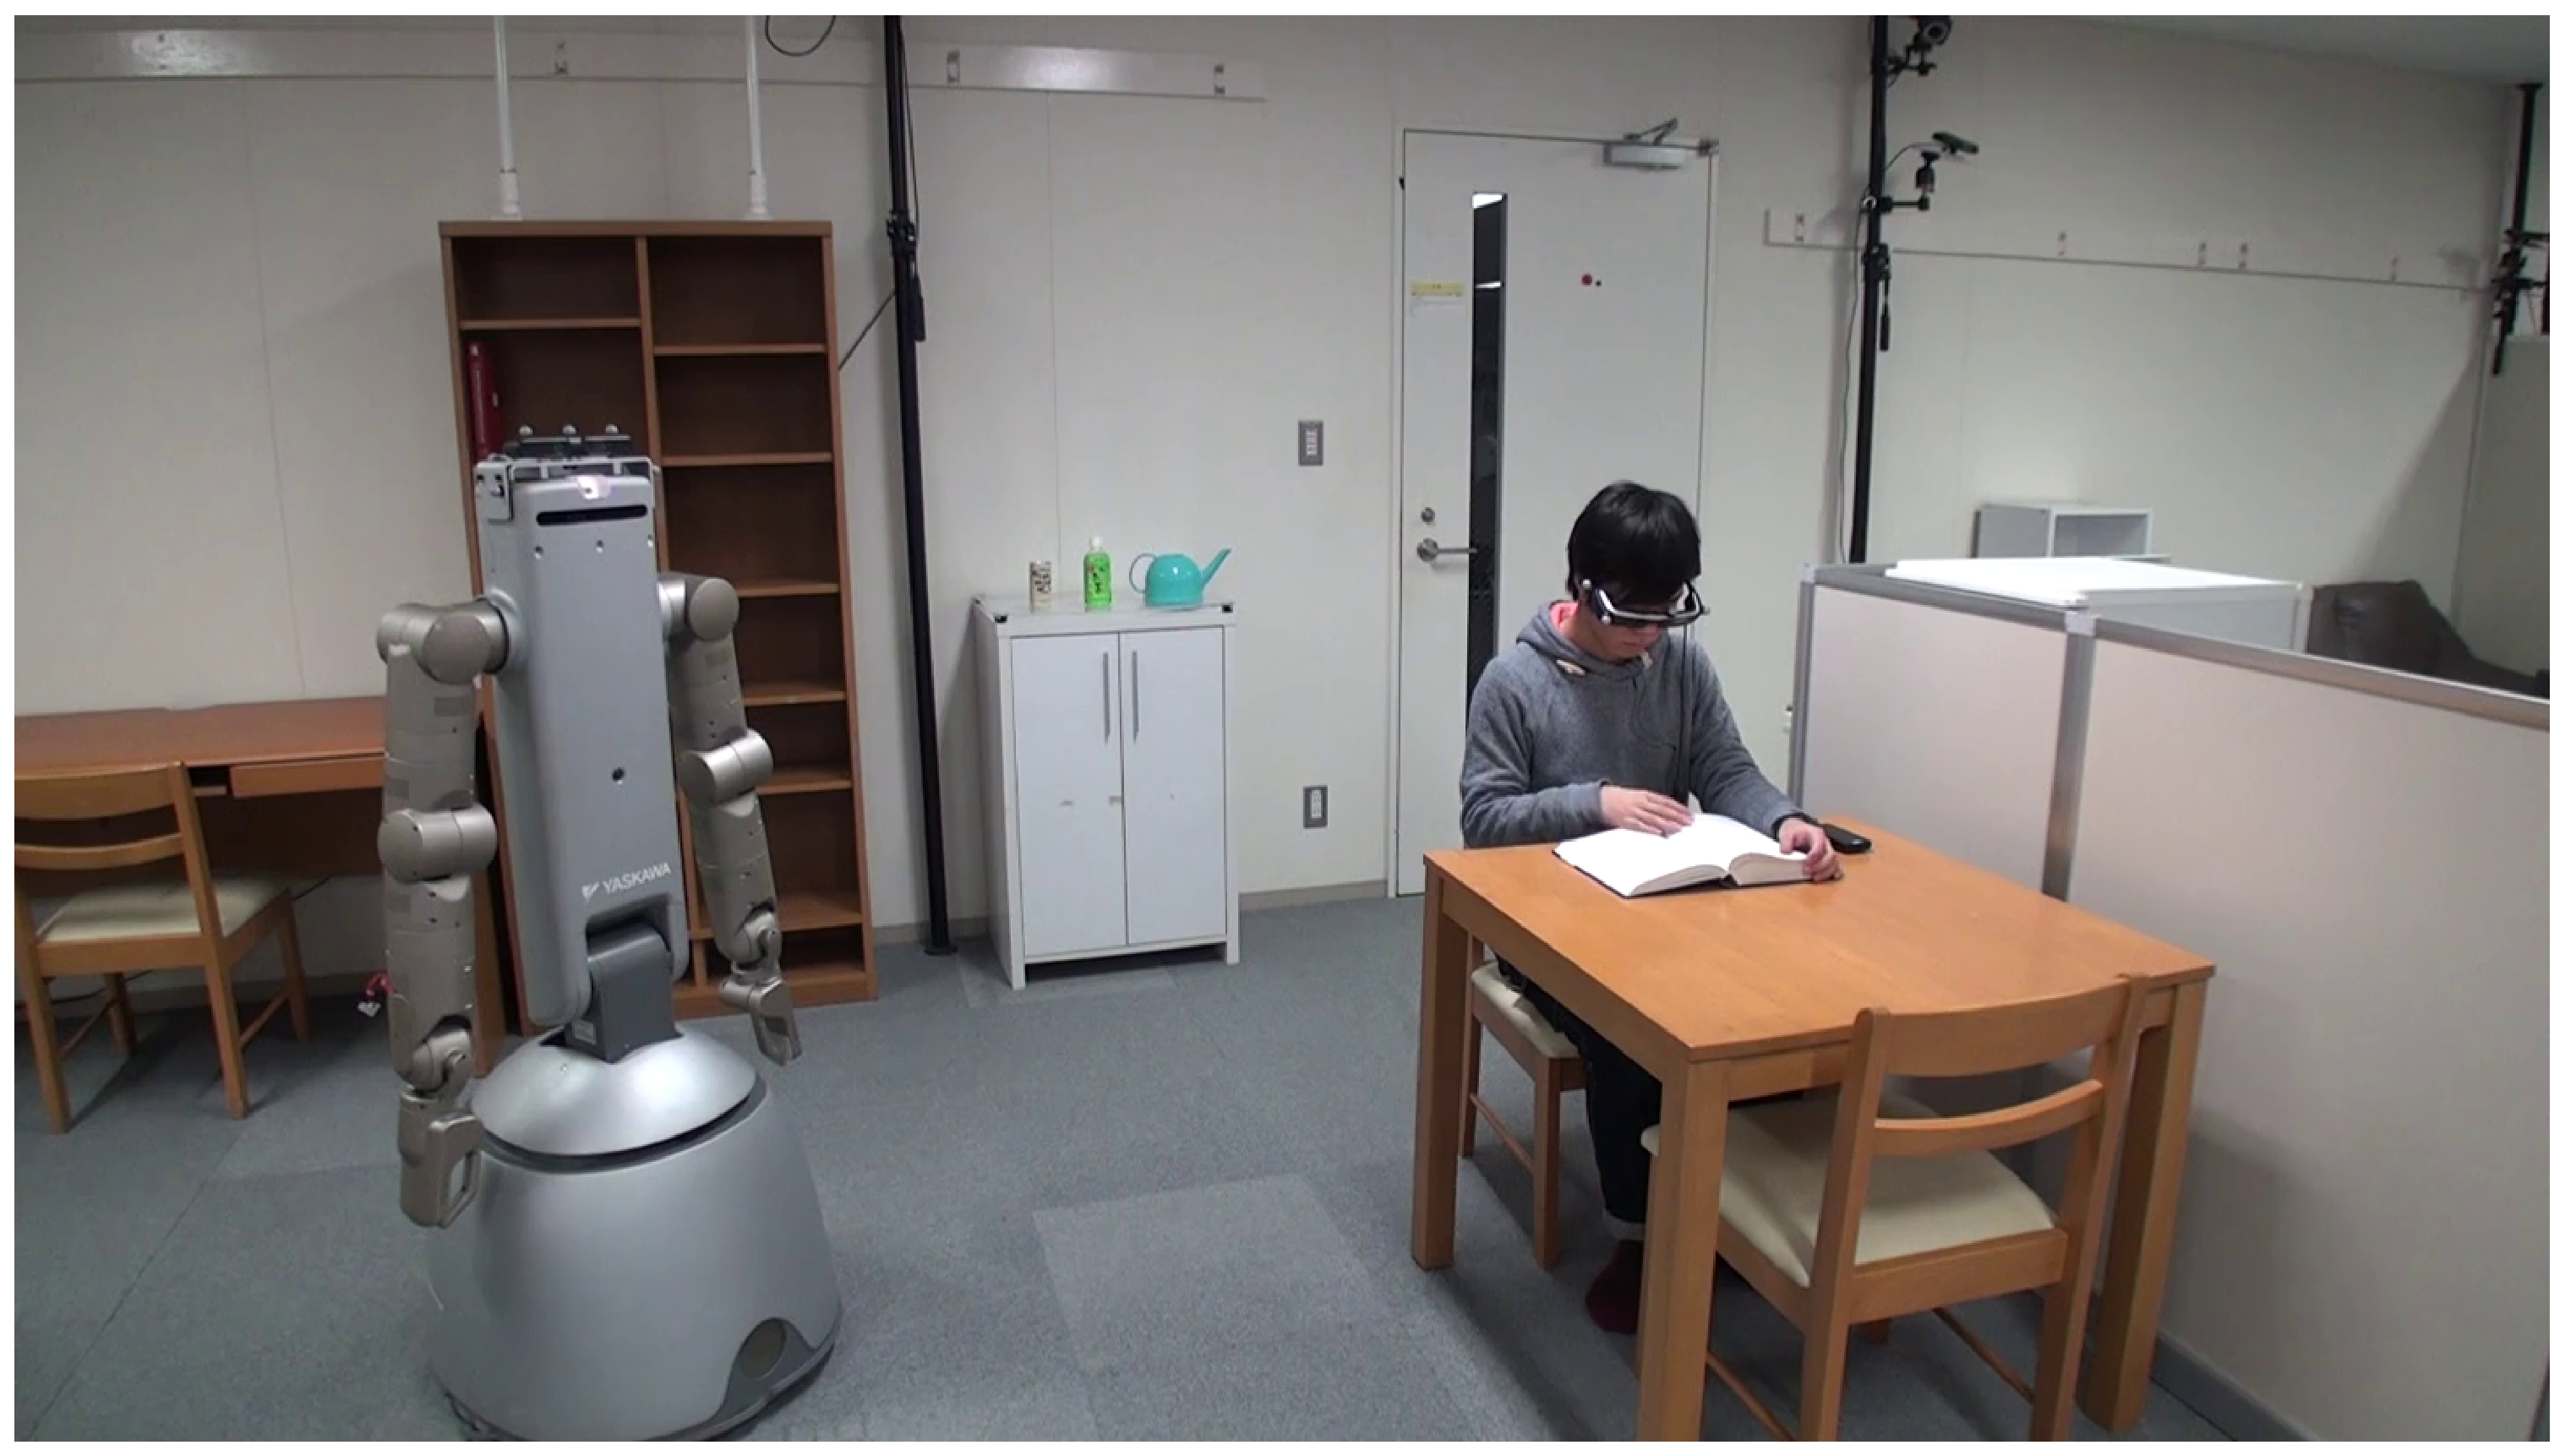
\includegraphics[height=40mm]{figure/experiment_2_water_1.eps}
    \end{center}
  \end{minipage}
%
  \begin{minipage}{0.5\textwidth}
    \begin{center}
      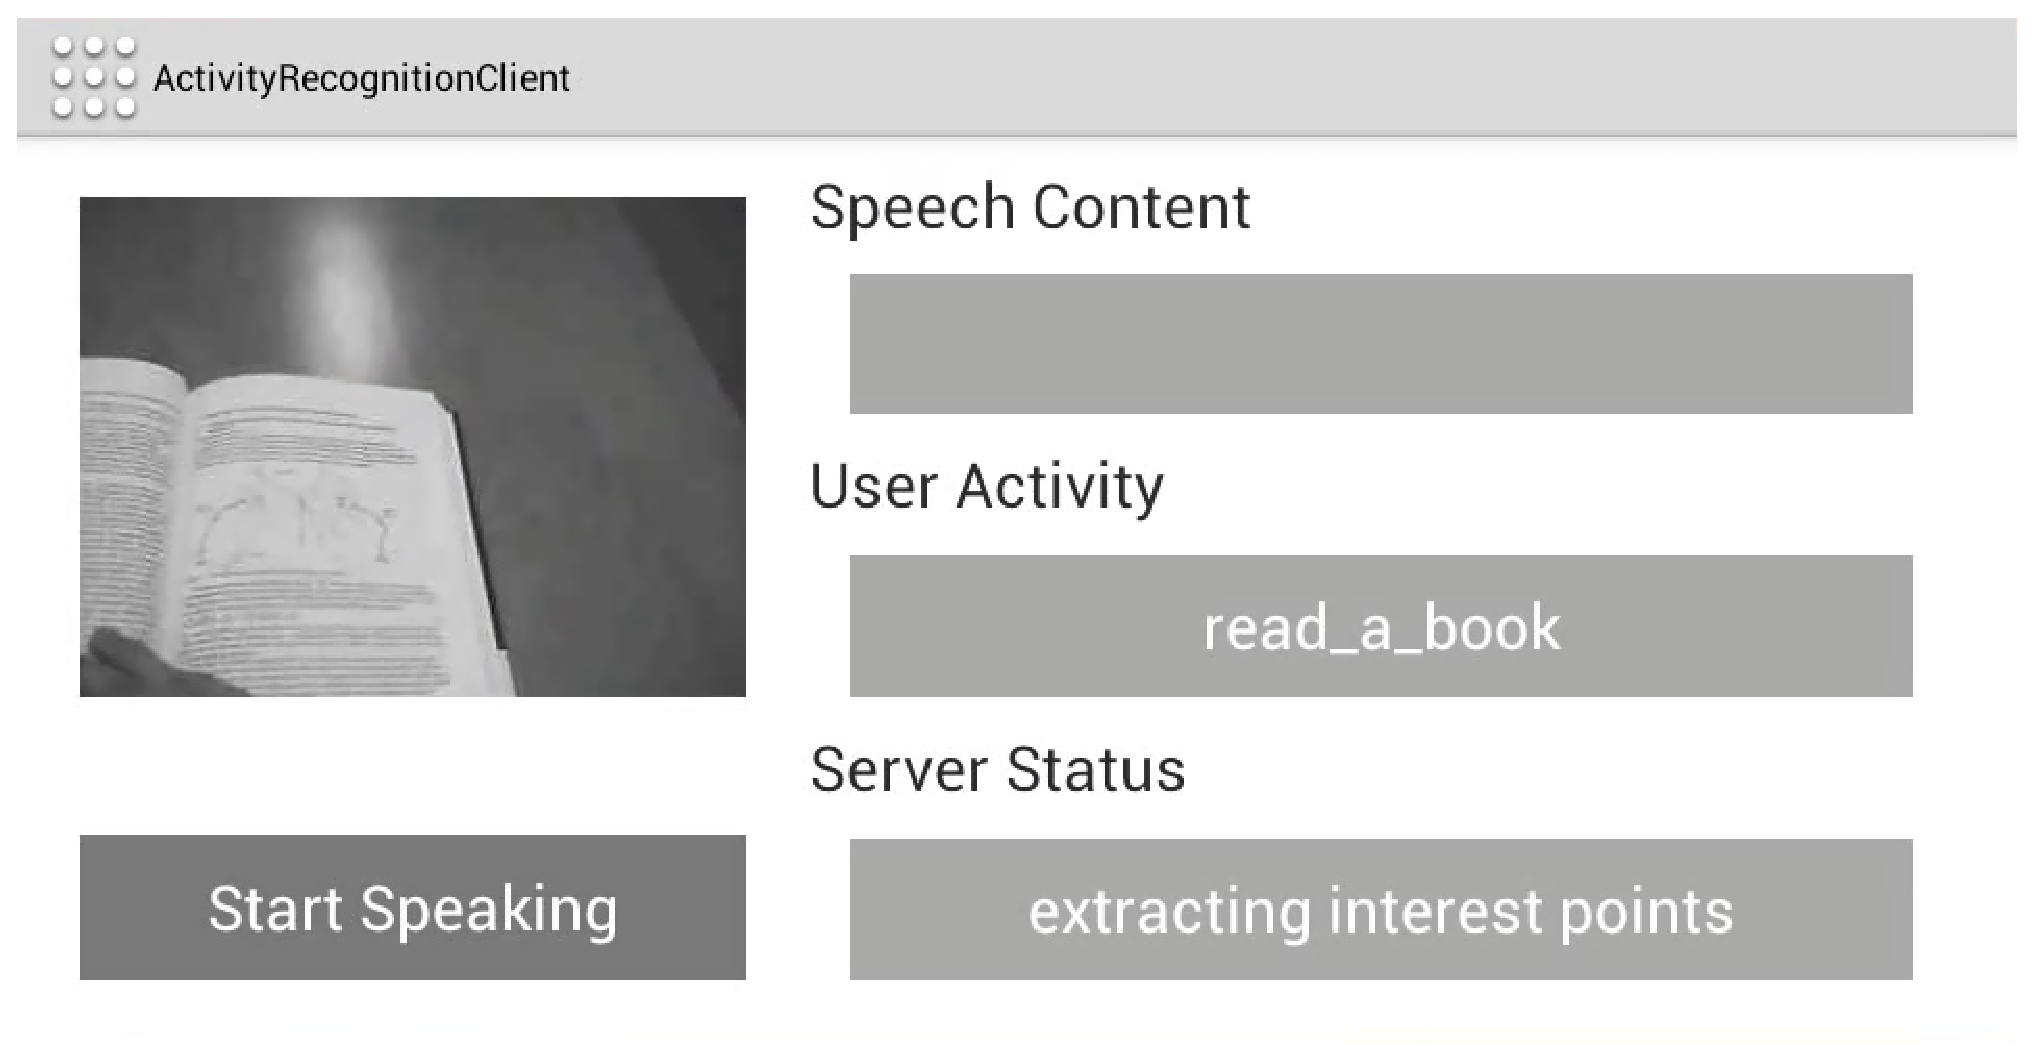
\includegraphics[height=40mm]{figure/experiment_2_water_1_a.eps}
    \end{center}
  \end{minipage}
%
\end{tabular}
\caption{読書している場合のサービス要求}
\label{fig:experiment_2_water_1}
\end{figure}

図{\ref{fig:experiment_2_water_2}}は,食事している場合の様子である.1人称視点から得た動画像は食事していると識別された.また,水の取り寄せを指示したところ「Would you like a green tea bottle ?」という応答を得た.
%
\vspace{5mm}
\begin{figure}[htbp]
\begin{tabular}{cc}
%
  \begin{minipage}{0.5\textwidth}
    \begin{center}
      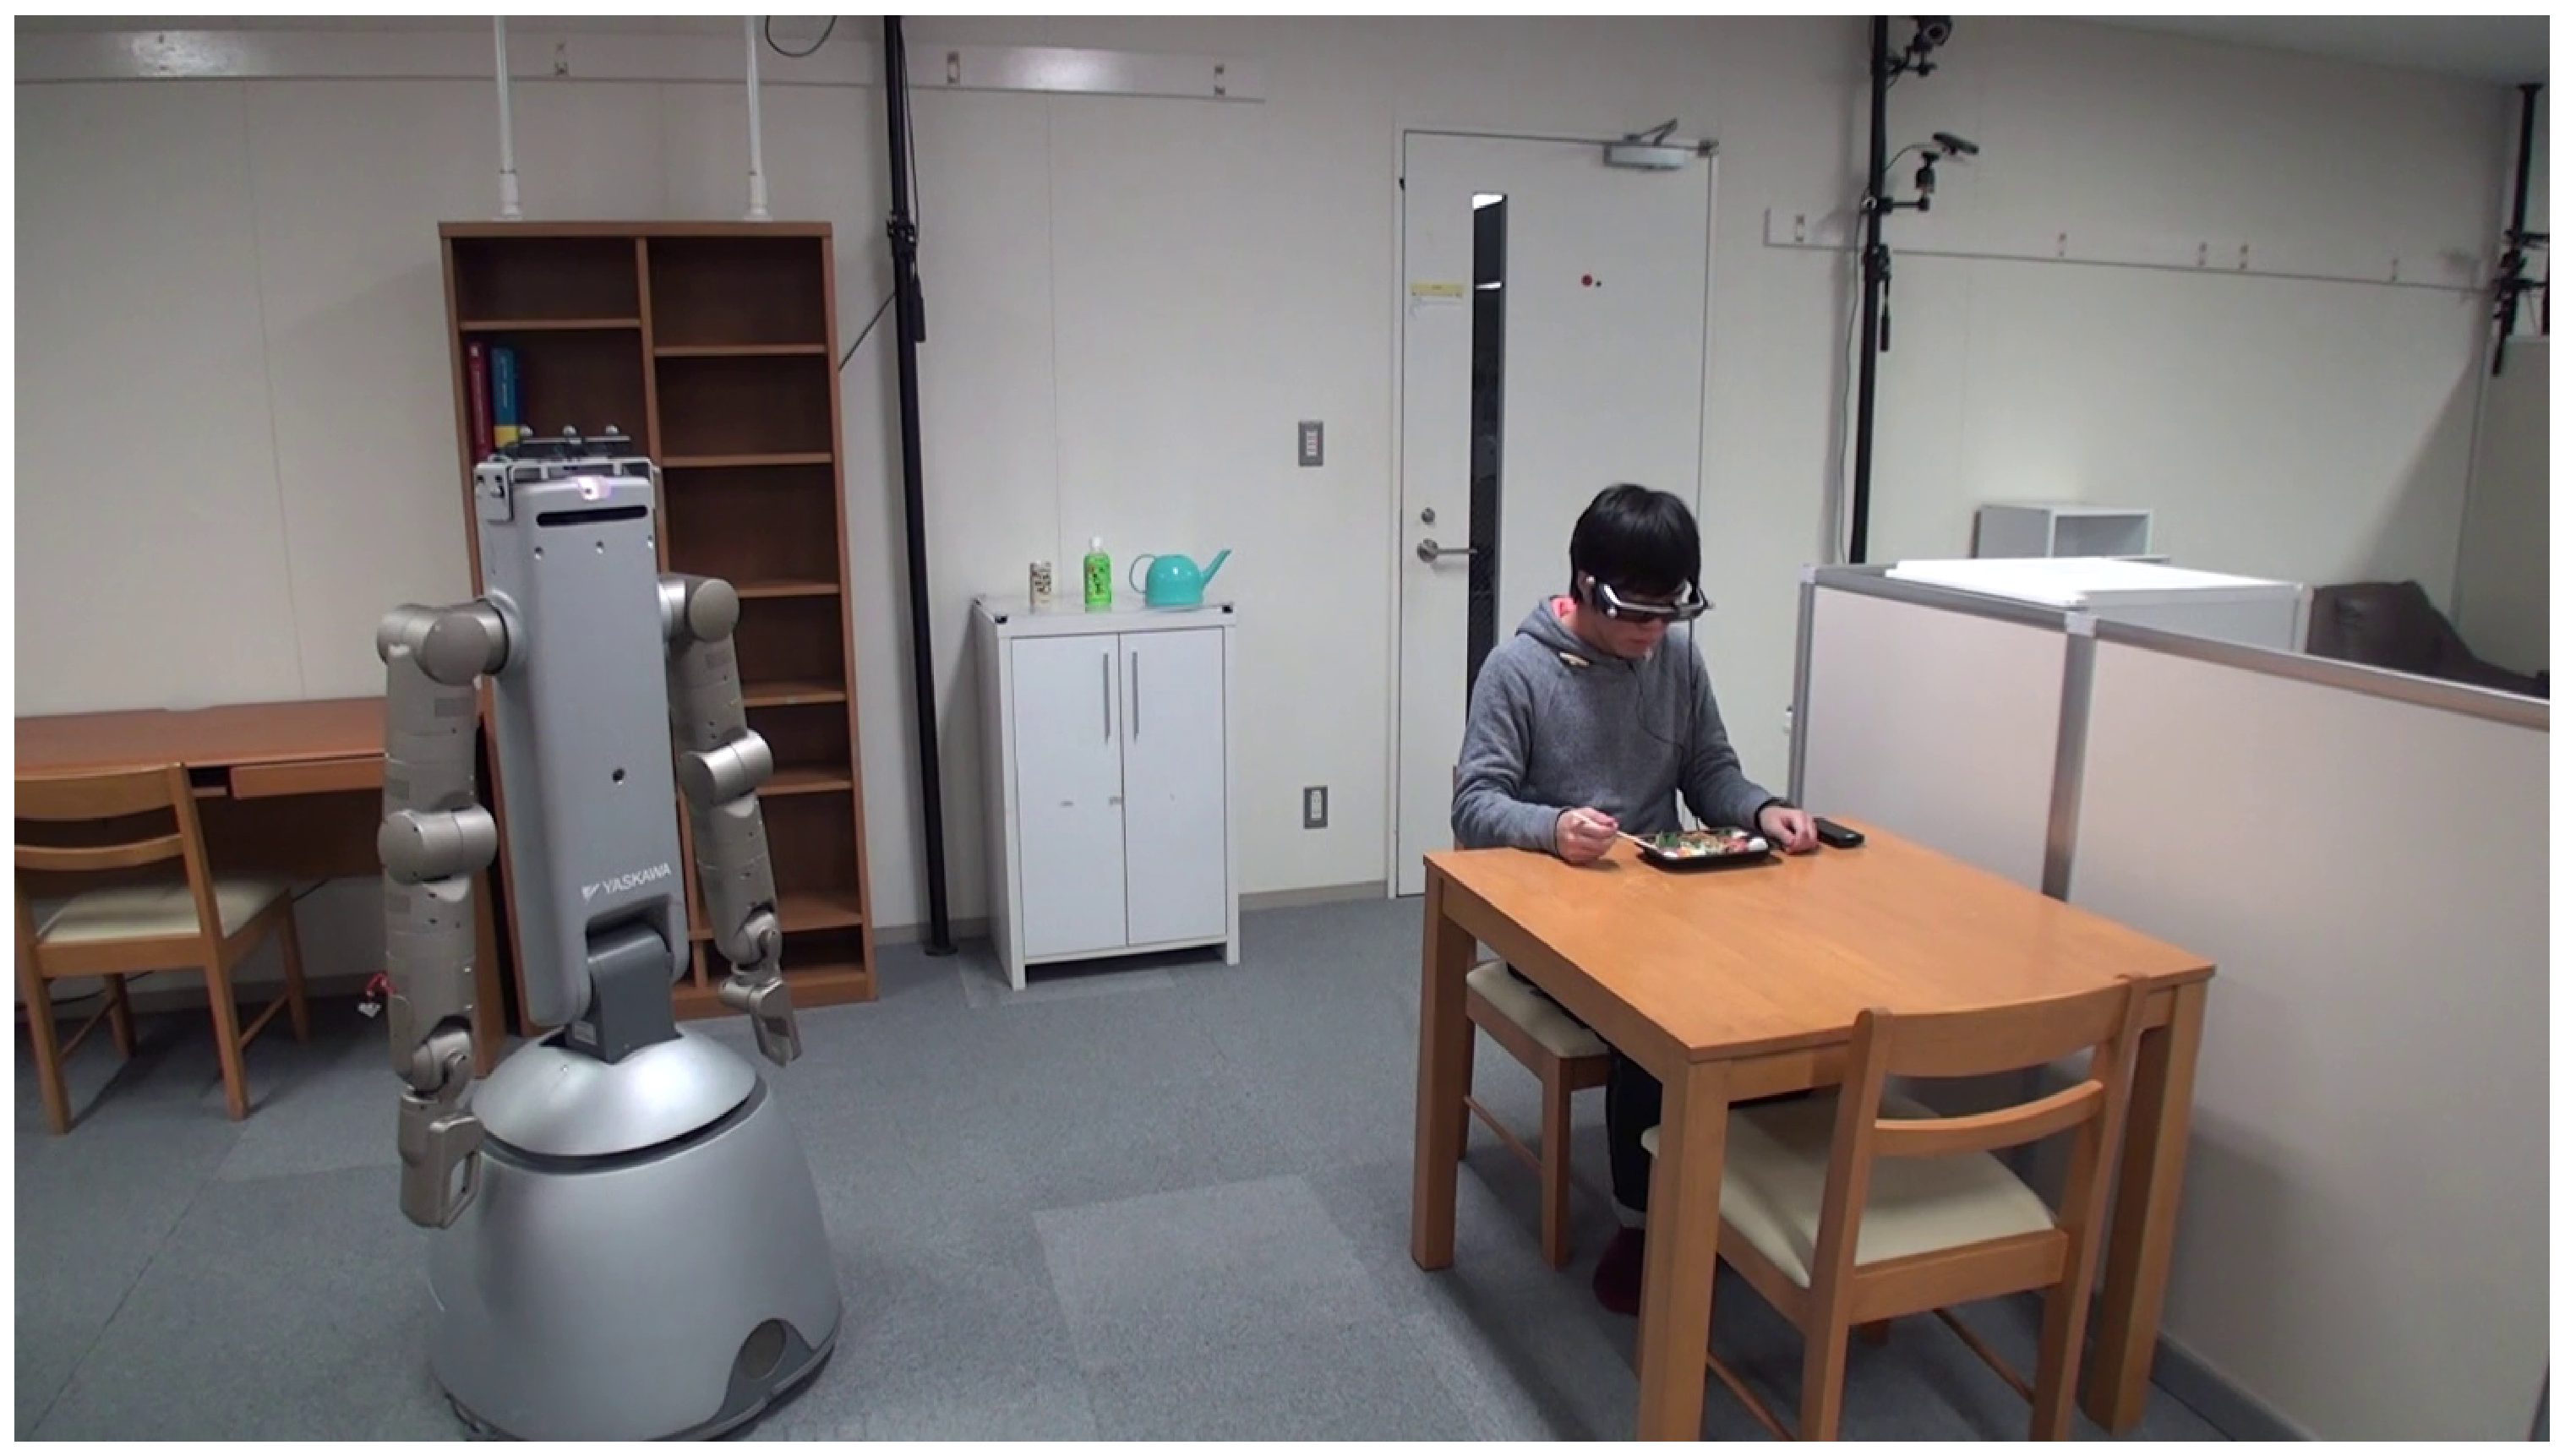
\includegraphics[height=40mm]{figure/experiment_2_water_2.eps}
    \end{center}
  \end{minipage}
%
  \begin{minipage}{0.5\textwidth}
    \begin{center}
      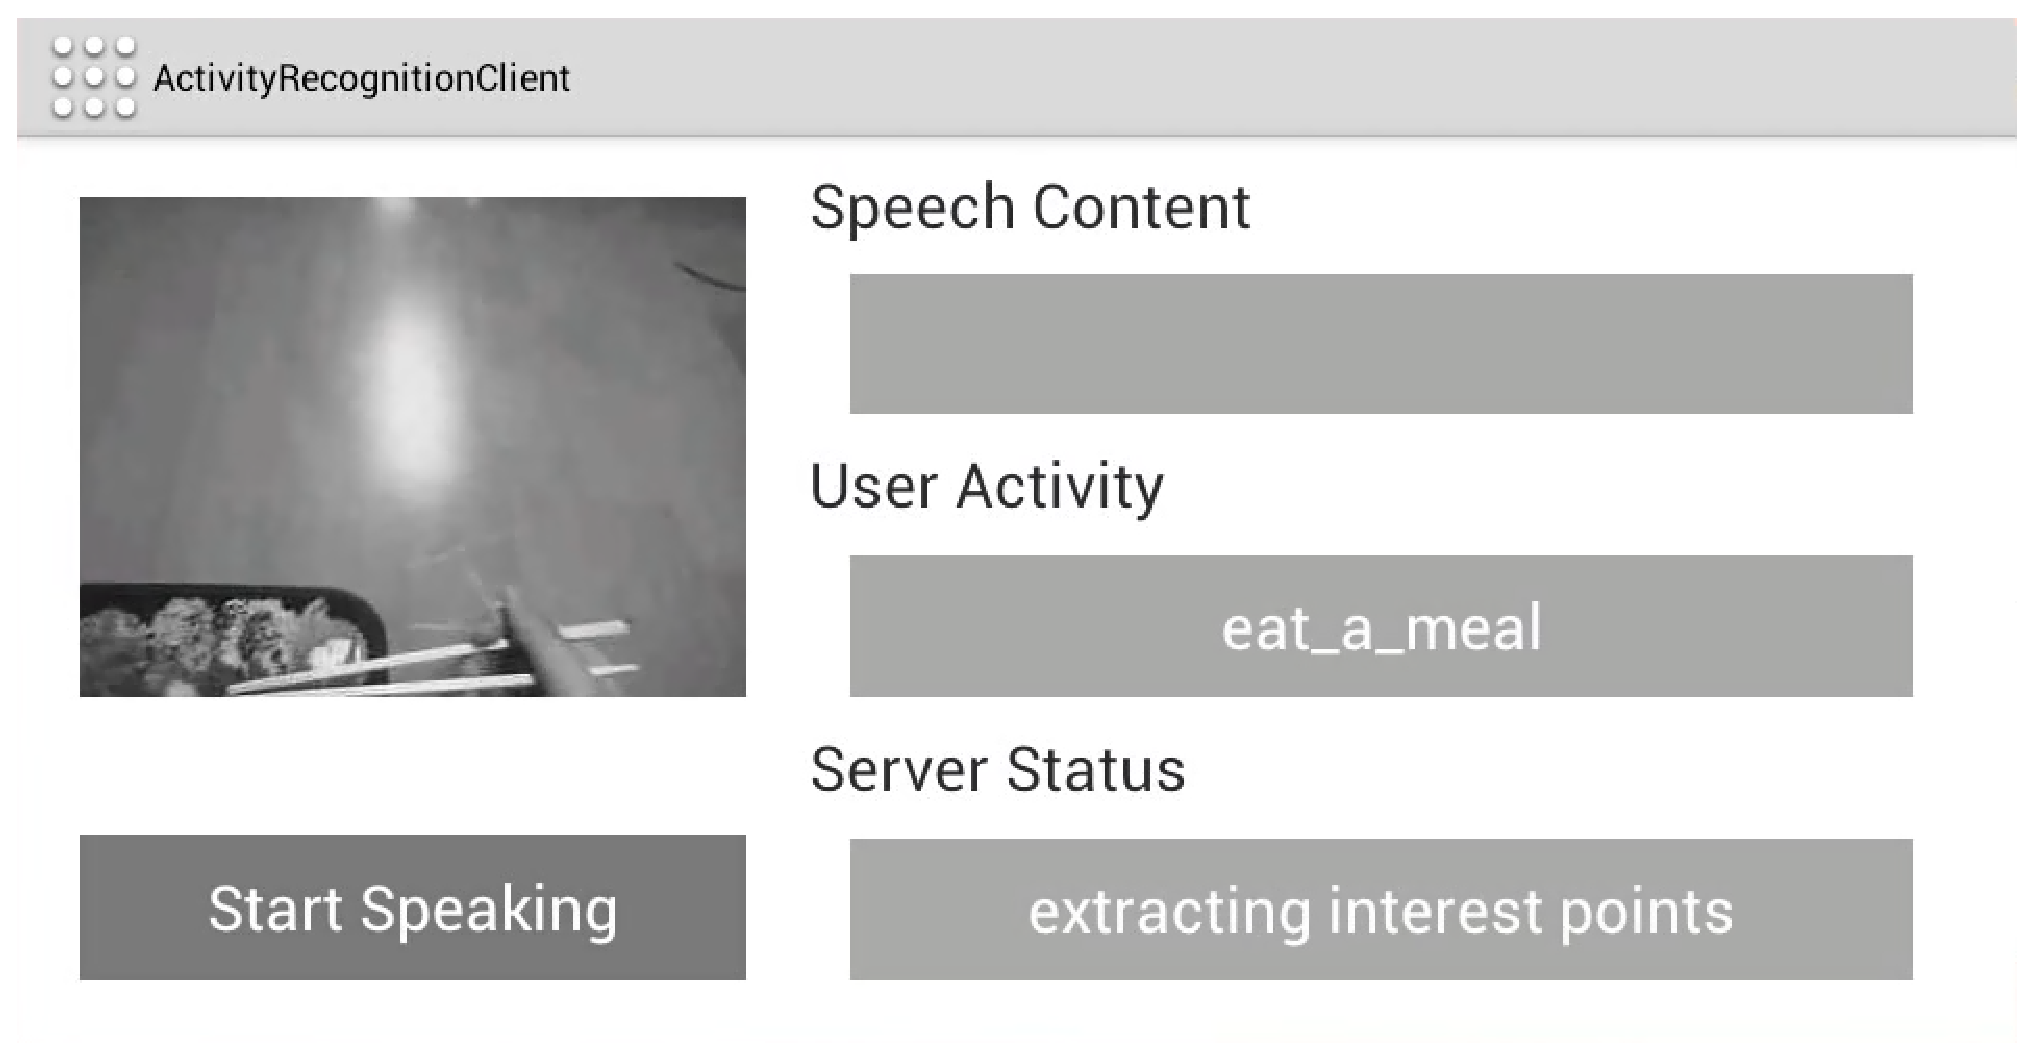
\includegraphics[height=40mm]{figure/experiment_2_water_2_a.eps}
    \end{center}
  \end{minipage}
%
\end{tabular}
\caption{食事している場合のサービス要求}
\label{fig:experiment_2_water_2}
\end{figure}

\newpage
図{\ref{fig:experiment_2_water_3}}は,植木を注視している場合の様子である.1人称視点から得た動画像は植木を注視していると識別された.また,水の取り寄せを指示したところ「Would you like a watering pot ?」という応答を得た.
%
\vspace{5mm}
\begin{figure}[htbp]
\begin{tabular}{cc}
%
  \begin{minipage}{0.5\textwidth}
    \begin{center}
      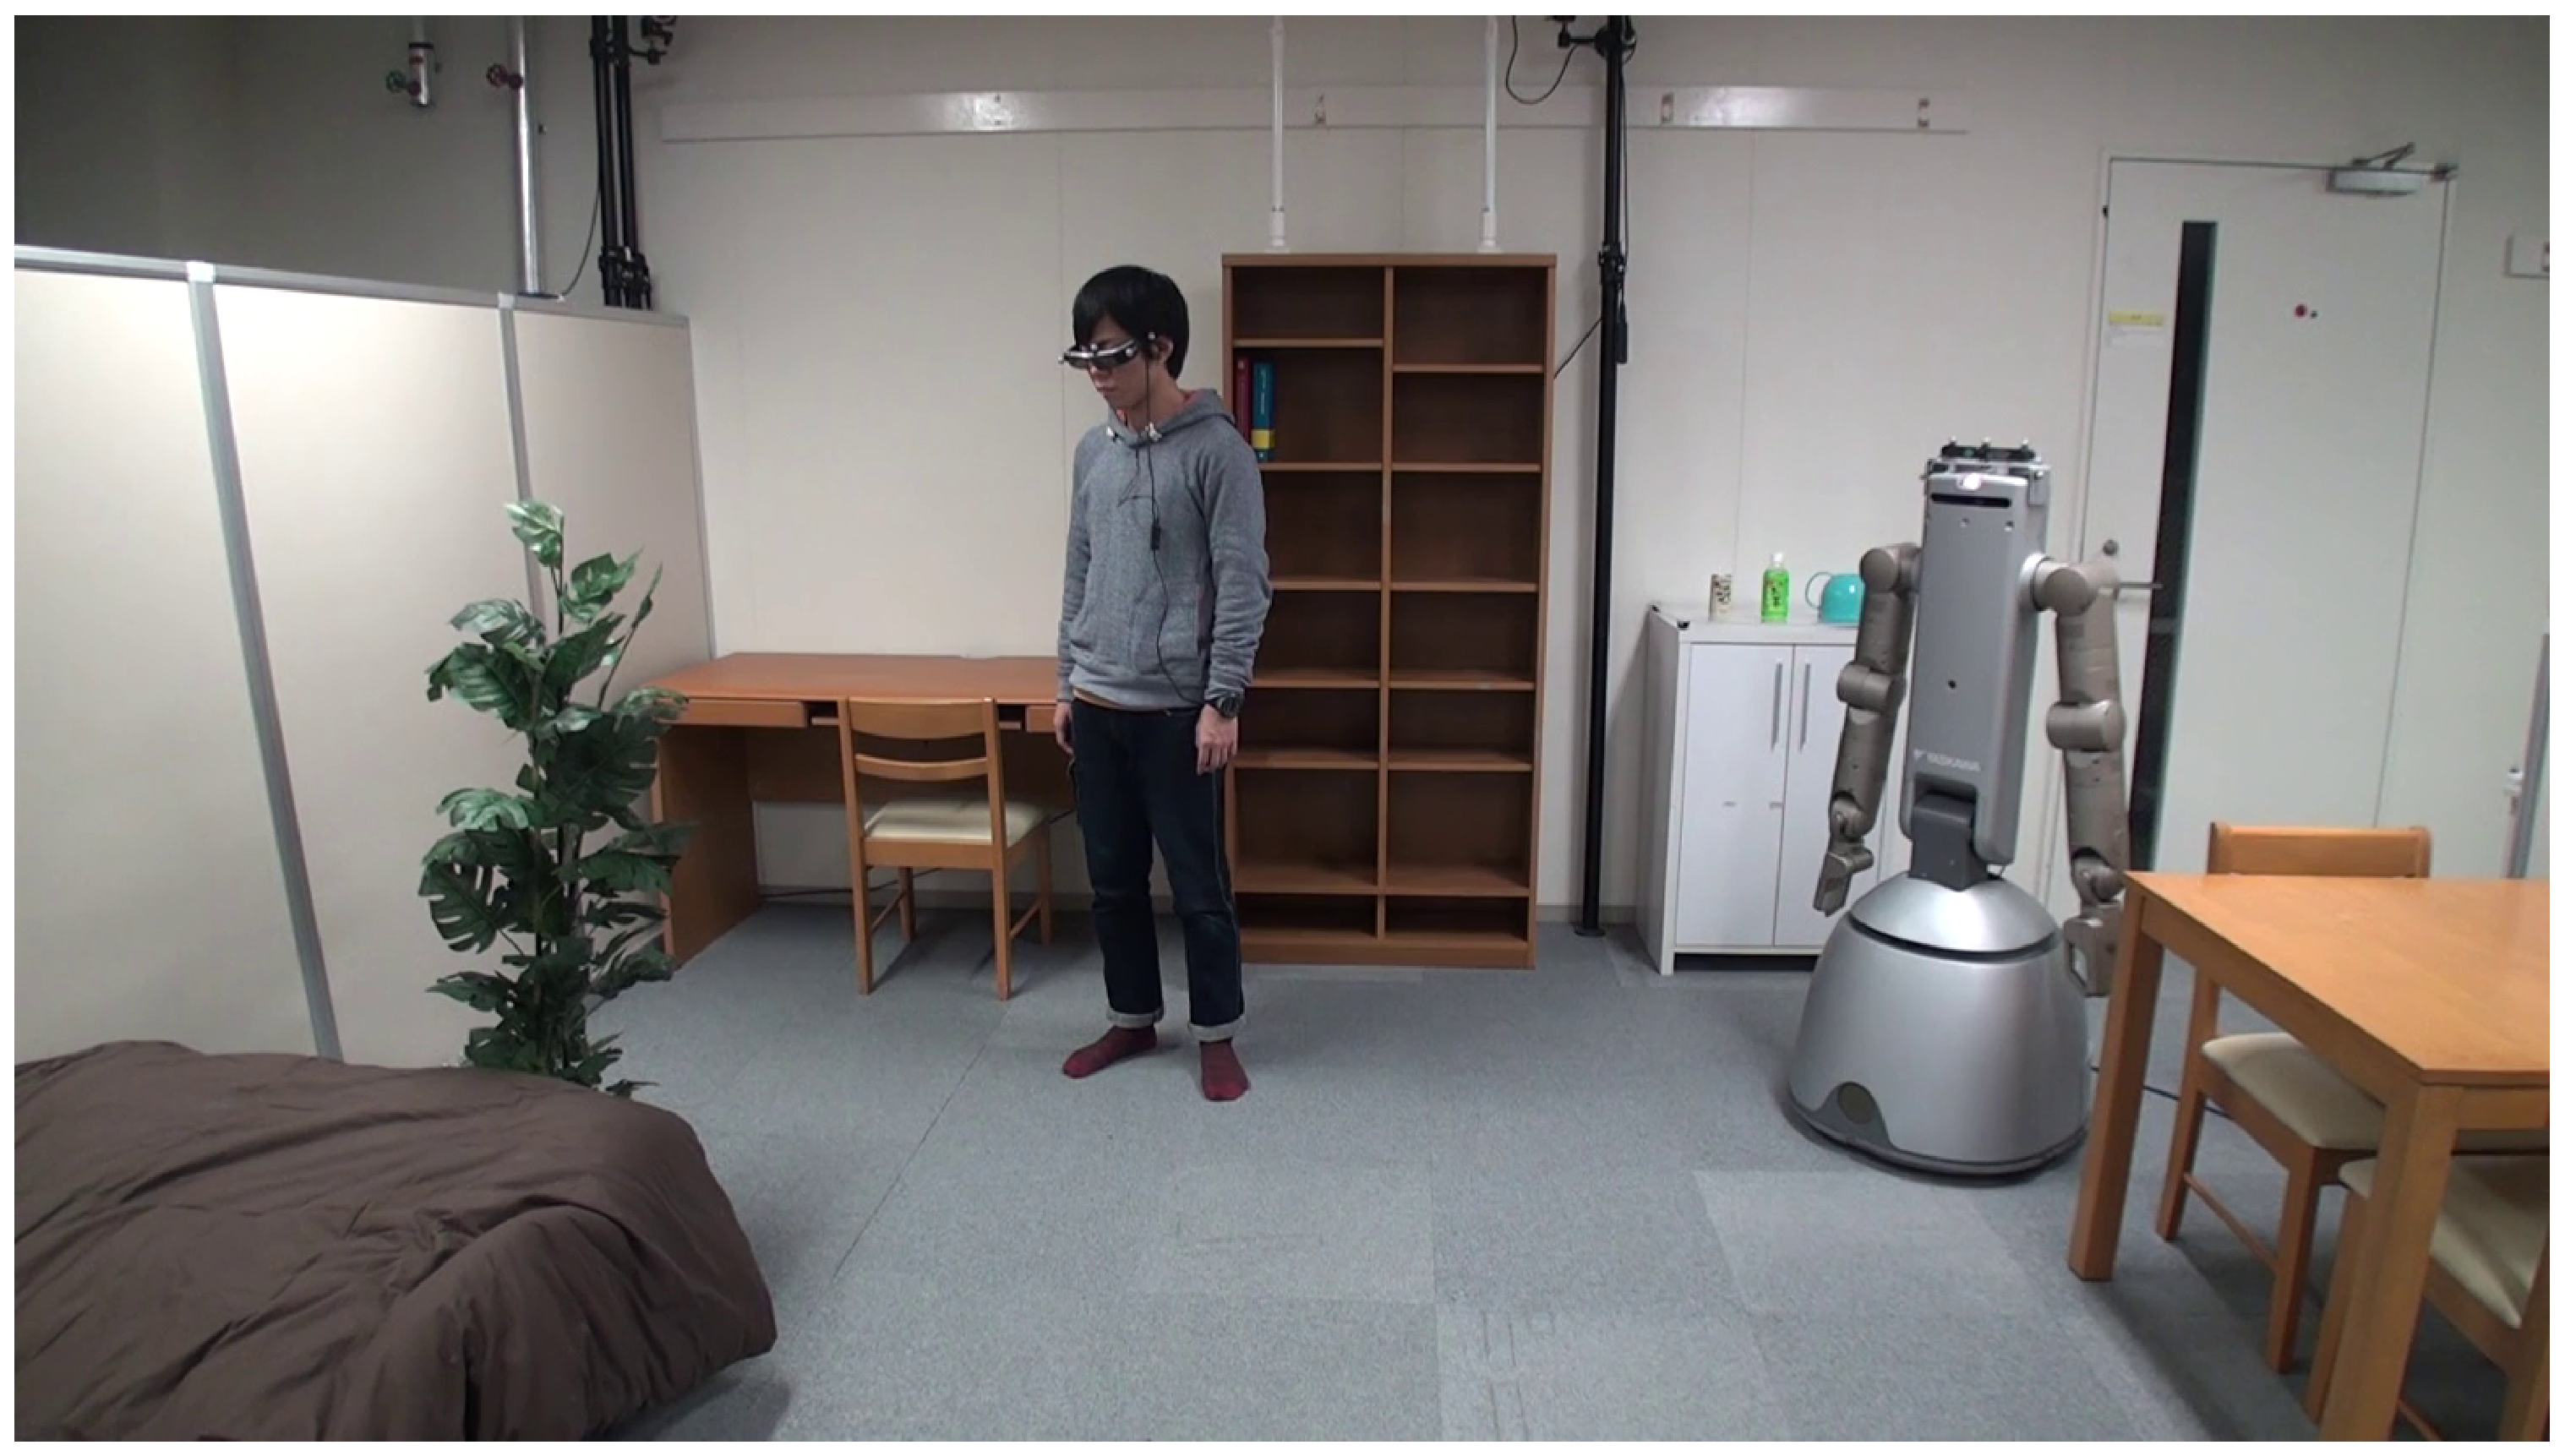
\includegraphics[height=40mm]{figure/experiment_2_water_3.eps}
    \end{center}
  \end{minipage}
%
  \begin{minipage}{0.5\textwidth}
    \begin{center}
      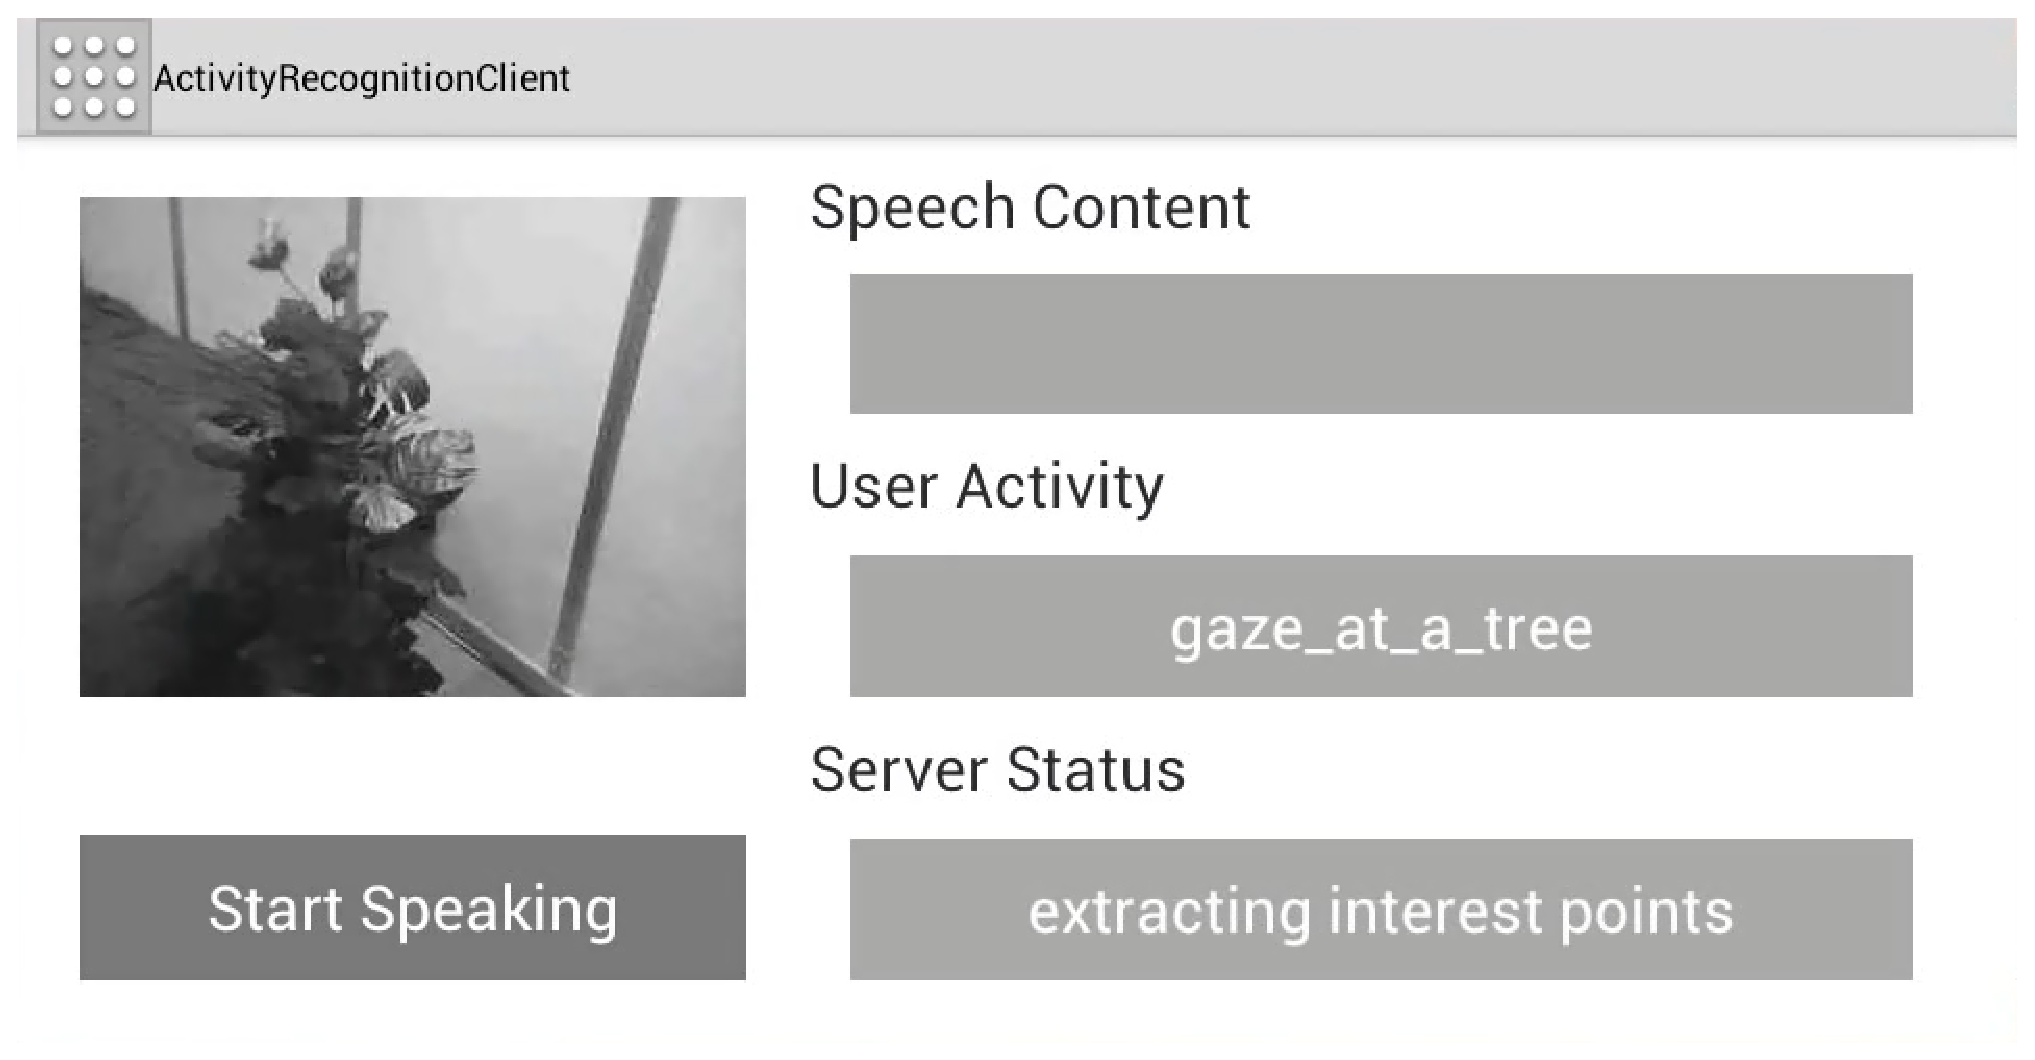
\includegraphics[height=40mm]{figure/experiment_2_water_3_a.eps}
    \end{center}
  \end{minipage}
%
\end{tabular}
\caption{植木を注視している場合のサービス要求}
\label{fig:experiment_2_water_3}
\end{figure}

いずれの行動もウェアラブルカメラから取得した1人称視点映像により正しく認識され,水の取り寄せ指示に対して行動情報に基づいた適切な物品の提示を行うことができた.

表{\ref{tb:experiment_2_result}}に,各行動が識別された際のSVMの推定事後確率と,行動情報によって複数候補がソーティングされた結果を示す.
「読書する」と「食事する」の推定事後確率は比較的高いが,「植木を注視する」は半分を下回った.
STIPで検出される時空間上の特徴点が少ないためであると考えられる.
また,「読書する」と「食事する」の優先順位に注目すると,1番目から3番目を飲料水が占め,4番目にジョーロが位置している.すなわち,候補全体で行動情報に基づいた適切なソーティングが行われていることが分かる.一方で,表{\ref{tb:experiment_2_result}}の中には,同じ優先順位となる物品が存在する.現段階においては,データベースに登録されているタグ情報が少ないため,「greentea\_bottle」と「soukentea\_bottle」のような同じカテゴリの物品に対しては優先順位の差が付かず,このような場合が生じてしまう.この問題に対しては,各物品と行動情報に結びつけたタグ情報の増強や,優先度を与える評価基準の変更などを行う必要がある.

\begin{table}[htbp]
  \begin{center}
  \caption{各行動における推定事後確率と候補物品の優先順位}
  \label{tb:experiment_2_result}
    \begin{tabular}{c|ccc} \bhline{1.2pt}
      行動 & 読書する & 食事する & 植木を注視する \\ \hline
      推定事後確率[\%] & 84.0 & 90.9 & 40.6 \\ \hline
      \multirow{4}{*}{優先順位}
      & 1. cancoffee & 1. greentea\_bottle & 1. watering\_pot \\
      & 2. greentea\_bottle & 1. soukentea\_bottle & 2. greentea\_bottle \\
      & 2. soukentea\_bottle & 2. cancoffee & 2. soukentea\_bottle \\
      & 3. watering\_pot & 3. watering\_pot & 2. cancoffee \\ \bhline{1.2pt}
    \end{tabular}
  \end{center}
\end{table}

\newpage
\subsection*{特定の行動をトリガとしたサービス}
検出対象の行動を行った場合の実験結果について述べる.次の図{\ref{fig:experiment_2_proactive_1}},図{\ref{fig:experiment_2_proactive_2}}に実環境の様子(左半分)とウェアラブルカメラのディスプレイ表示(右半分)を示す.

図{\ref{fig:experiment_2_proactive_1}}は,サービスロボットを注視している場合の様子である.1人称視点から得た動画像は,SVMの推定事後確率98.9%でサービスロボットを注視していると識別され,直後にサービスロボットから「May I help you ?」という音声を確認した.
%
\vspace{5mm}
\begin{figure}[htbp]
\begin{tabular}{cc}
%
  \begin{minipage}{0.5\textwidth}
    \begin{center}
      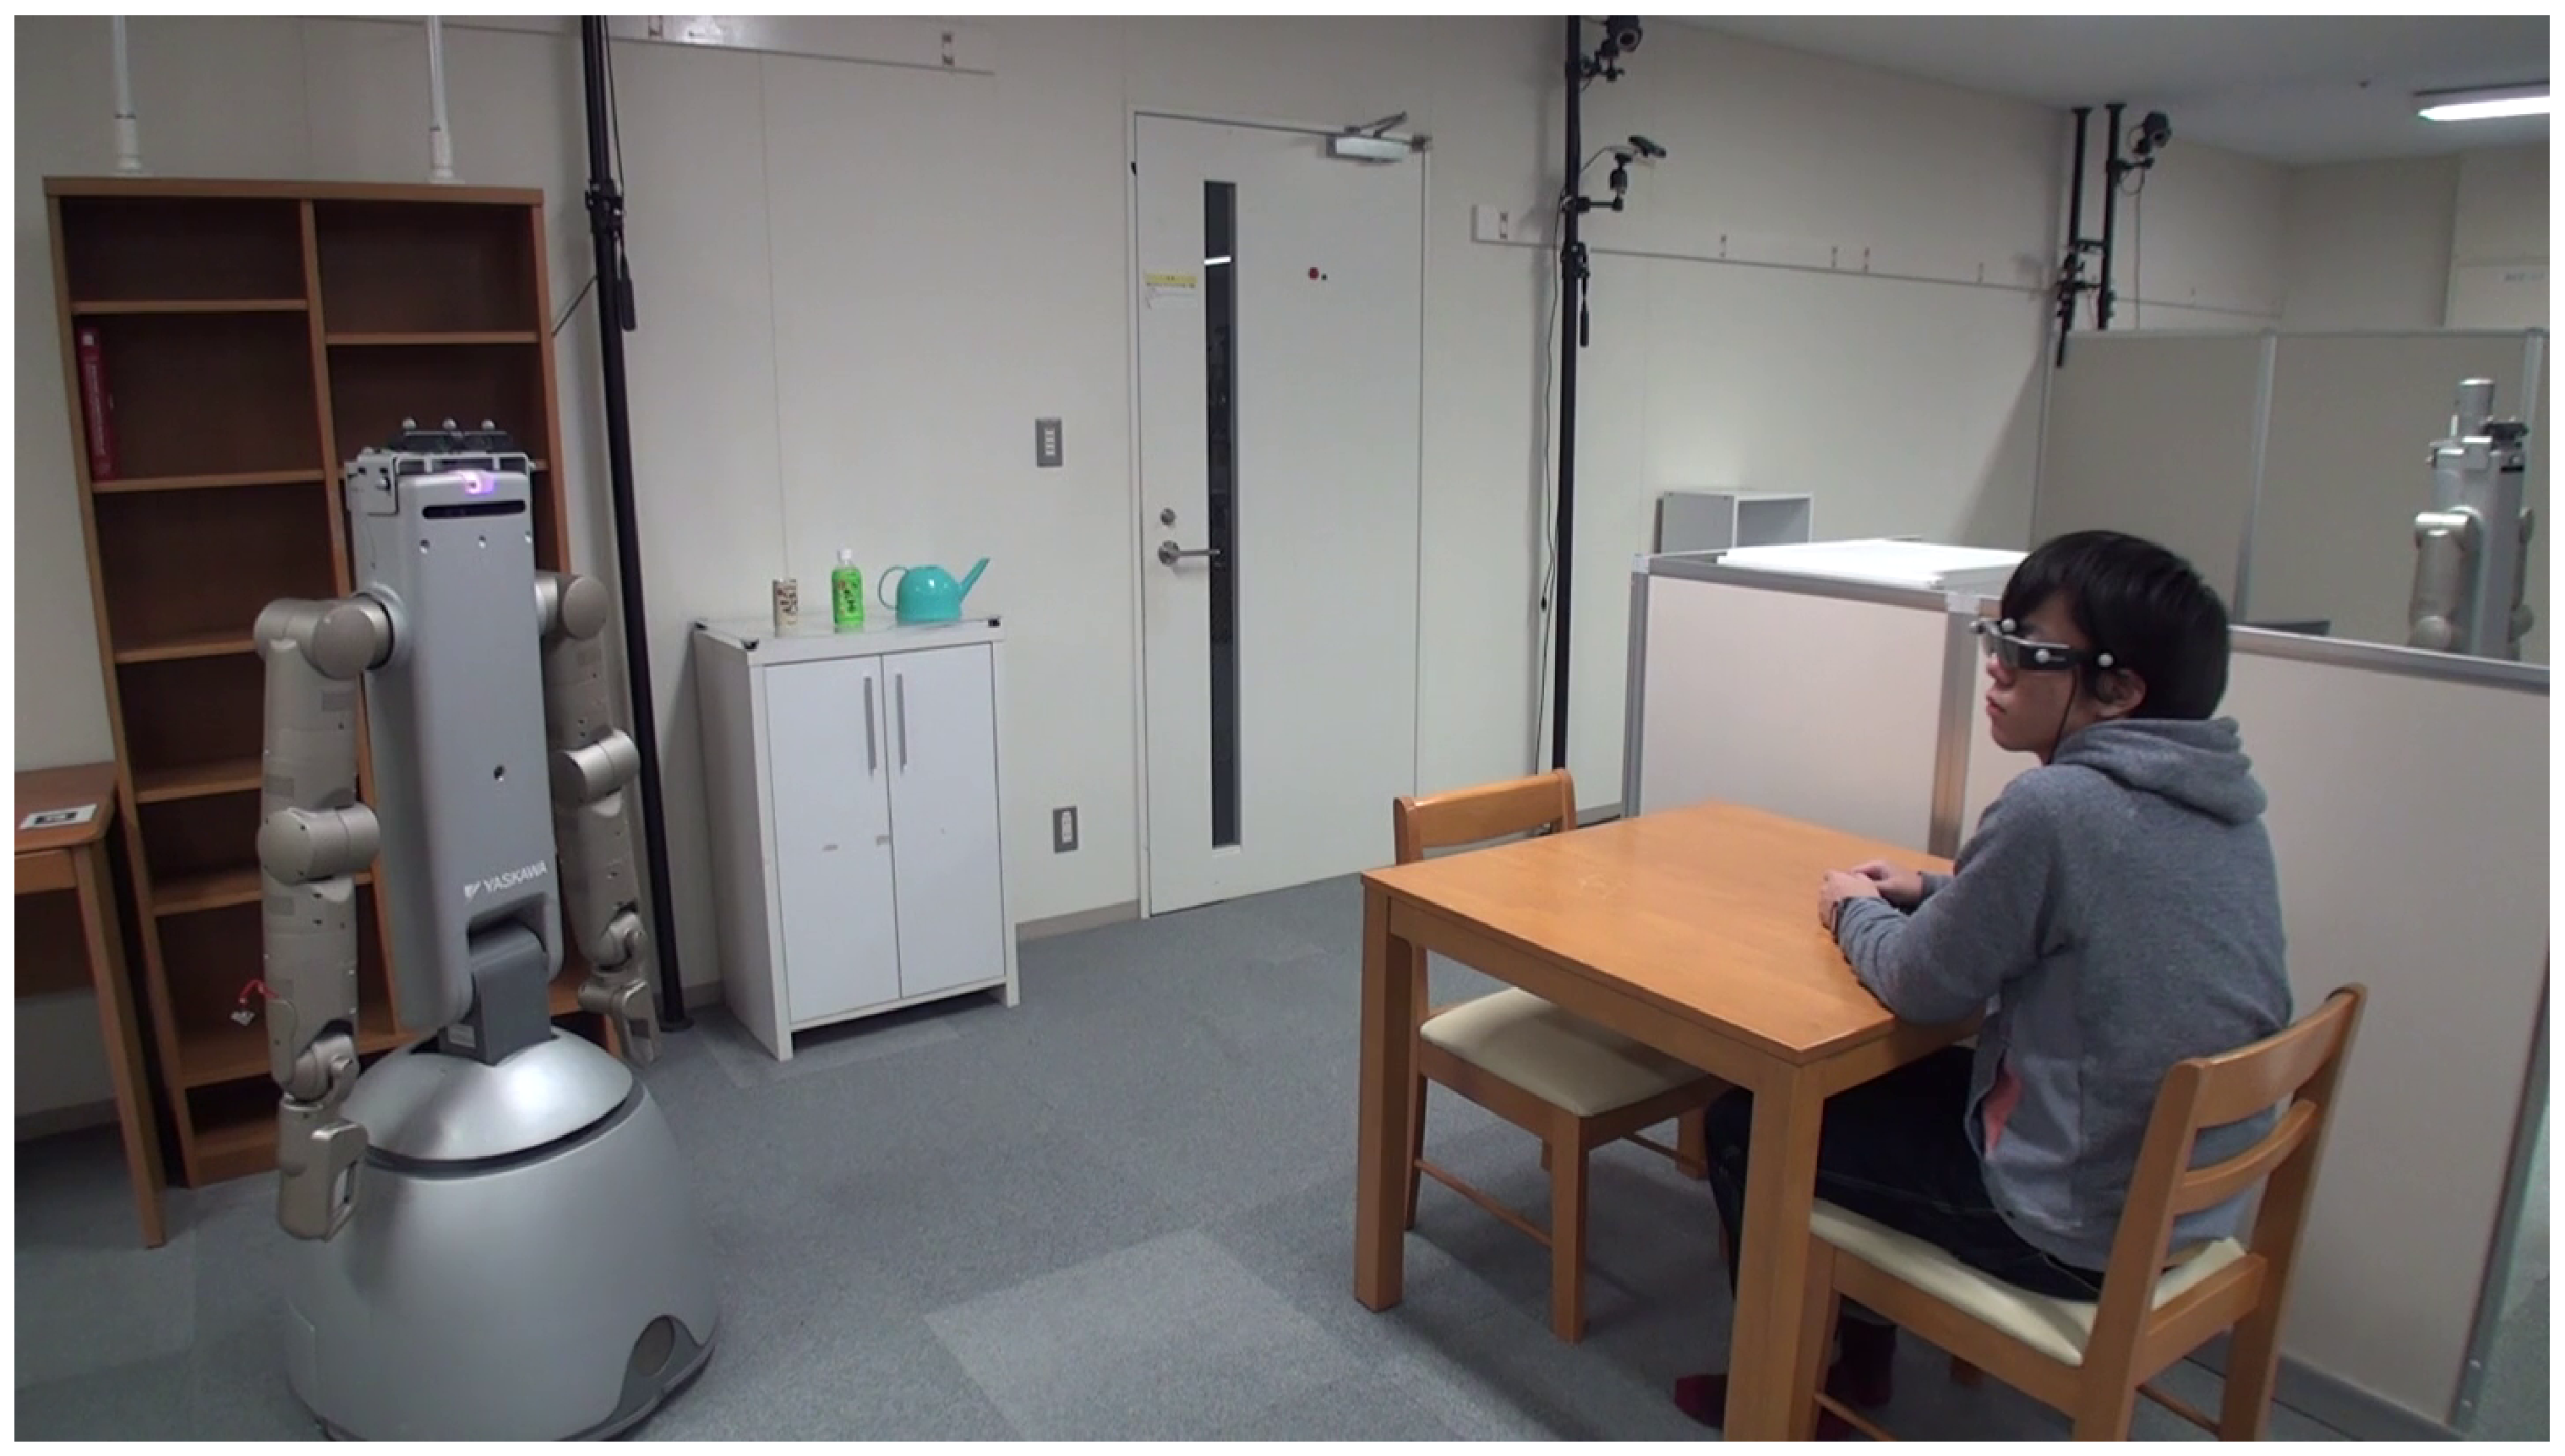
\includegraphics[height=40mm]{figure/experiment_2_proactive_1.eps}
    \end{center}
  \end{minipage}
%
  \begin{minipage}{0.5\textwidth}
    \begin{center}
      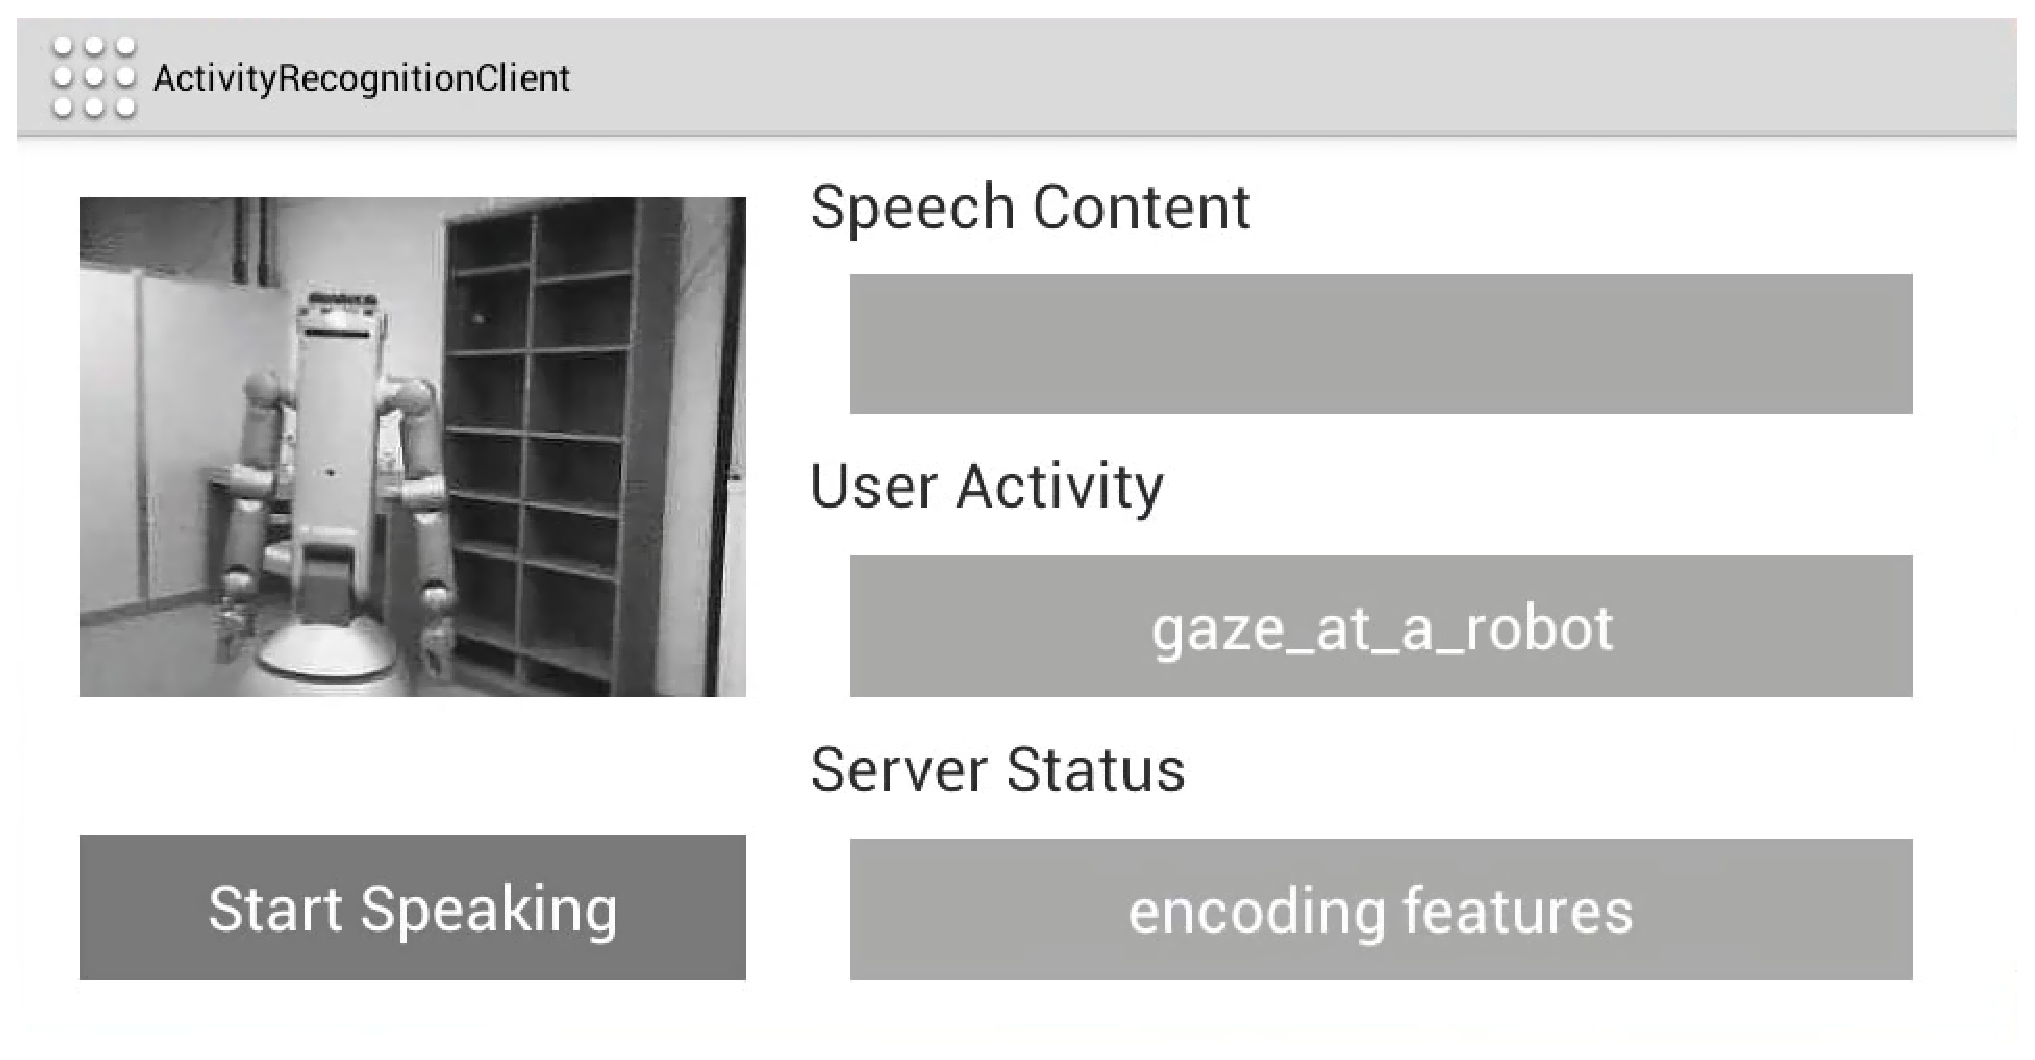
\includegraphics[height=40mm]{figure/experiment_2_proactive_1_a.eps}
    \end{center}
  \end{minipage}
%
\end{tabular}
\caption{サービスロボットを注視している場合}
\label{fig:experiment_2_proactive_1}
\end{figure}

図{\ref{fig:experiment_2_proactive_2}}は,辺りを見回している場合の様子である.1人称視点から得た動画像は,SVMの推定事後確率86.0%で辺りを見回していると識別され,直後にサービスロボットから「Are you looking for anything ?」という音声を確認した.
%
\vspace{5mm}
\begin{figure}[htbp]
\begin{tabular}{cc}
%
  \begin{minipage}{0.5\textwidth}
    \begin{center}
      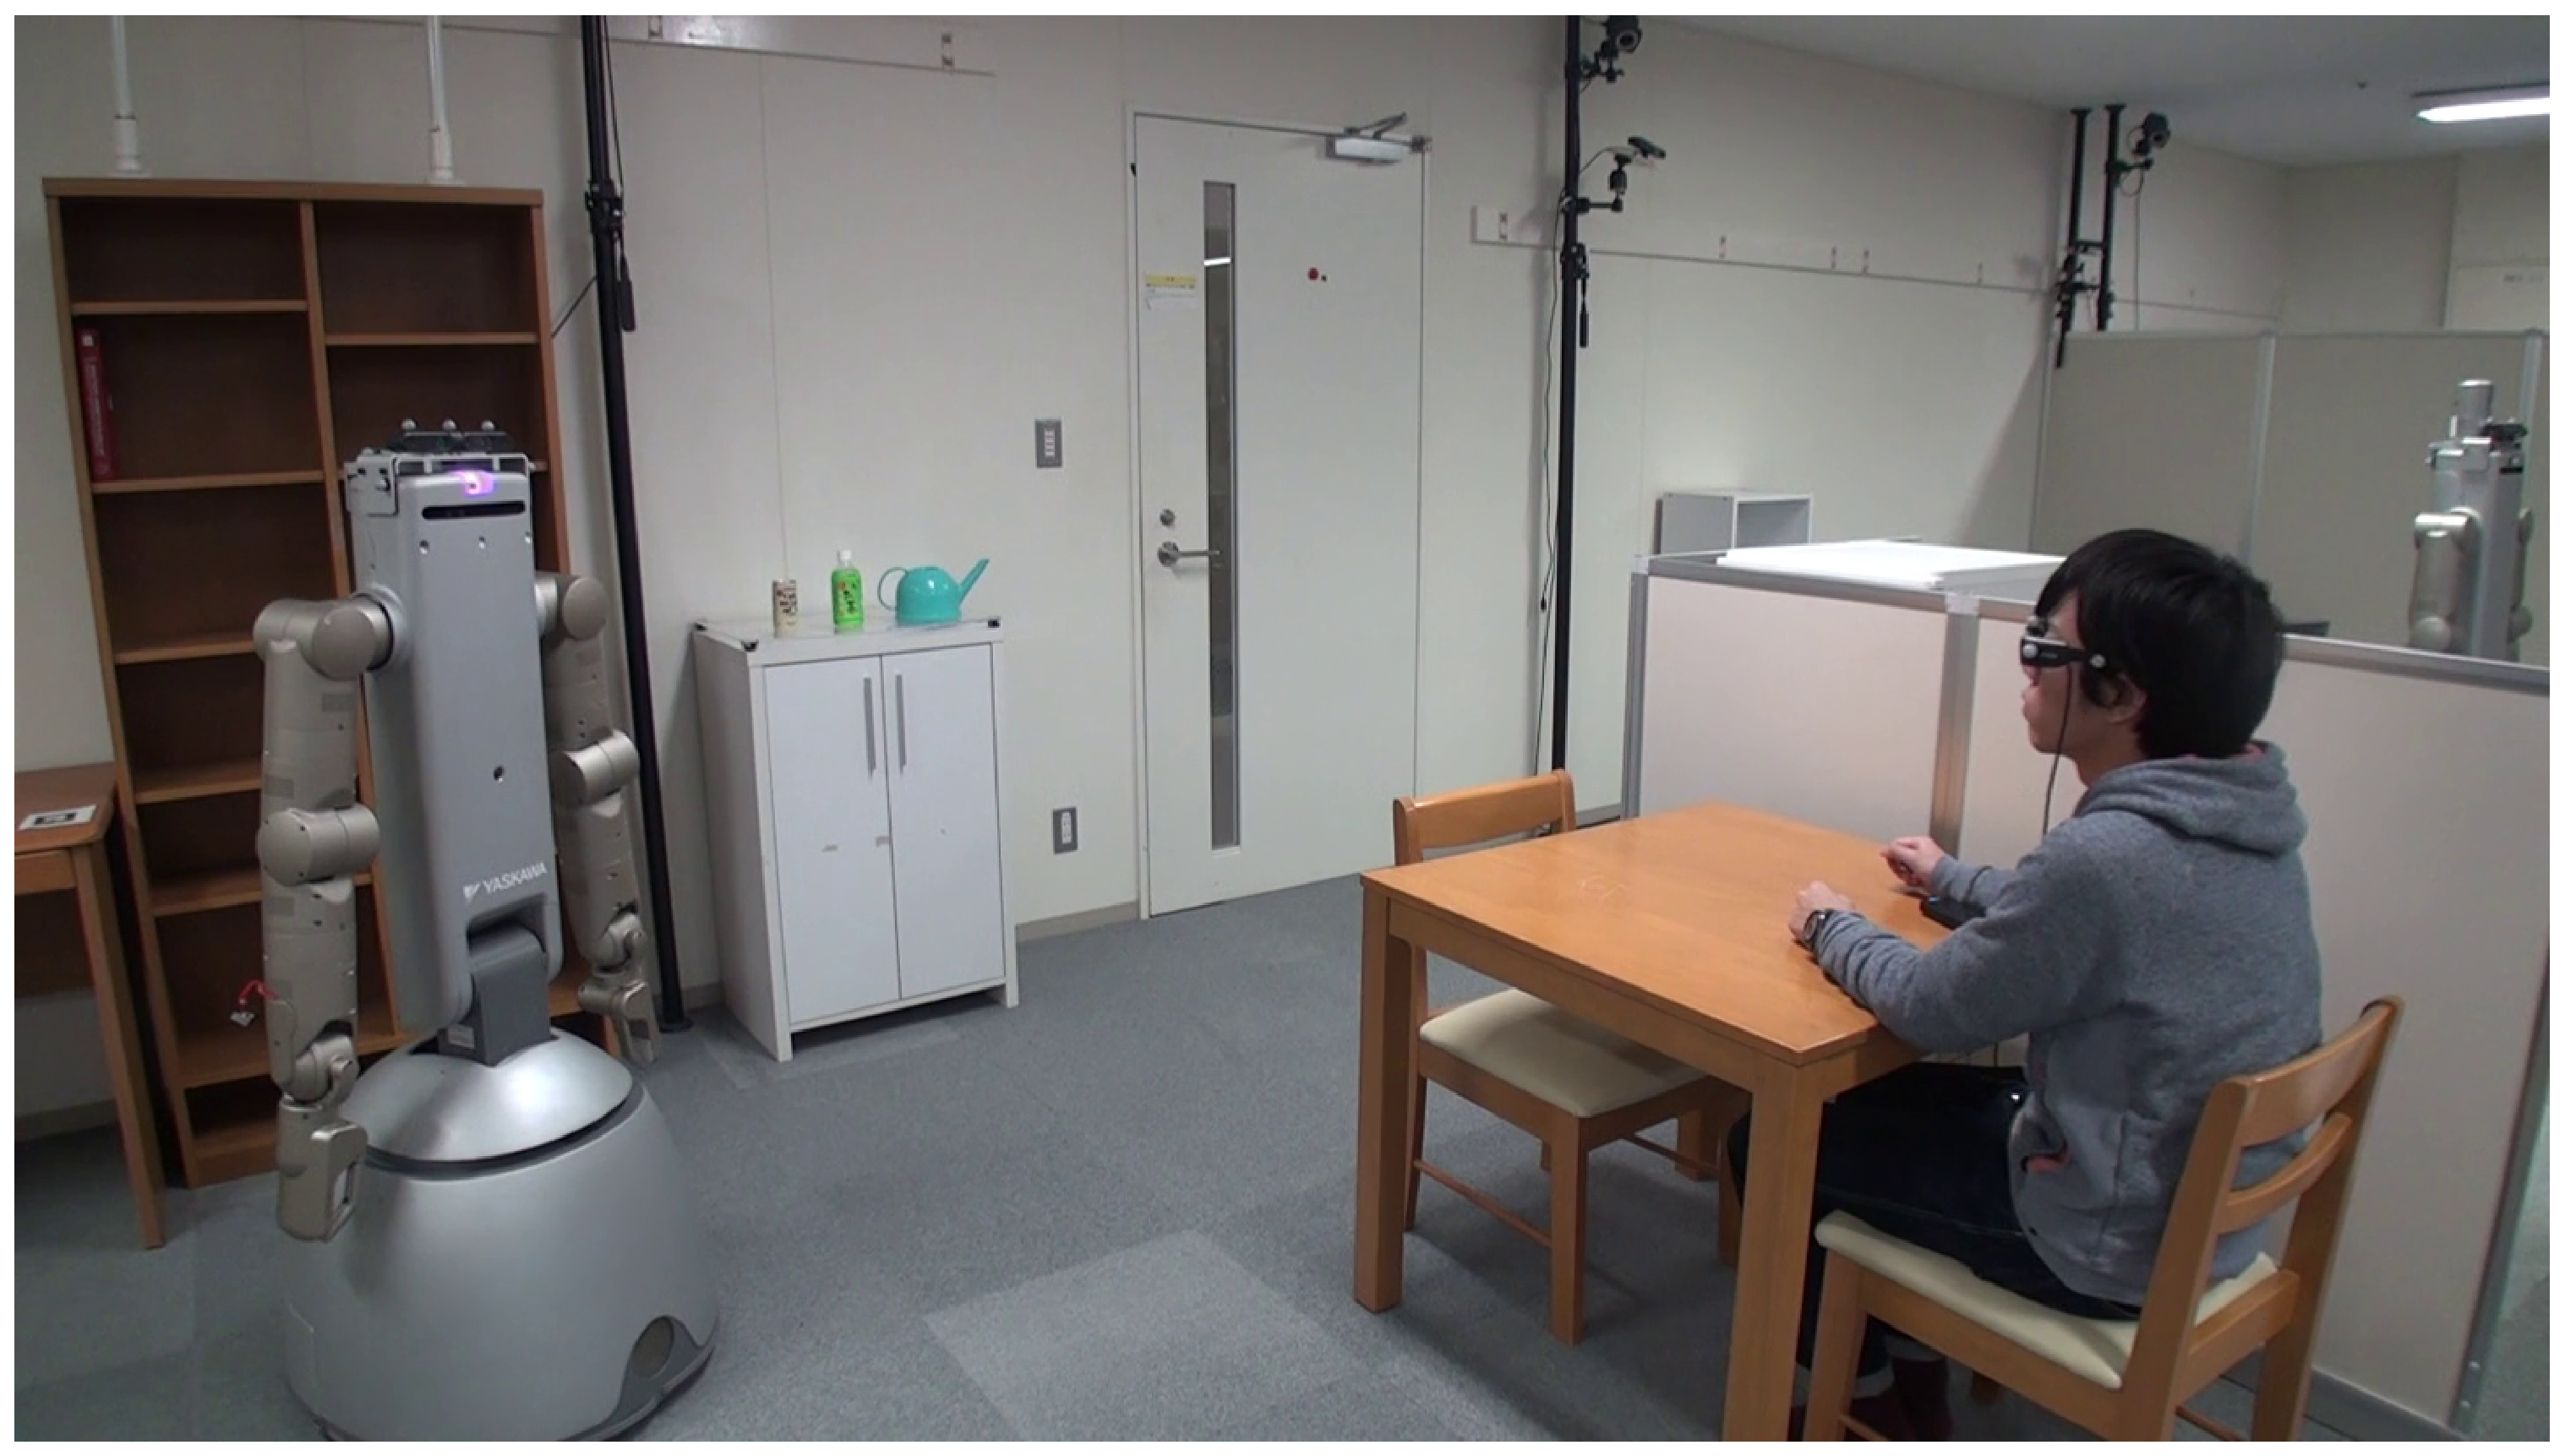
\includegraphics[width=75mm]{figure/experiment_2_proactive_2.eps}
    \end{center}
  \end{minipage}
%
  \begin{minipage}{0.5\textwidth}
    \begin{center}
      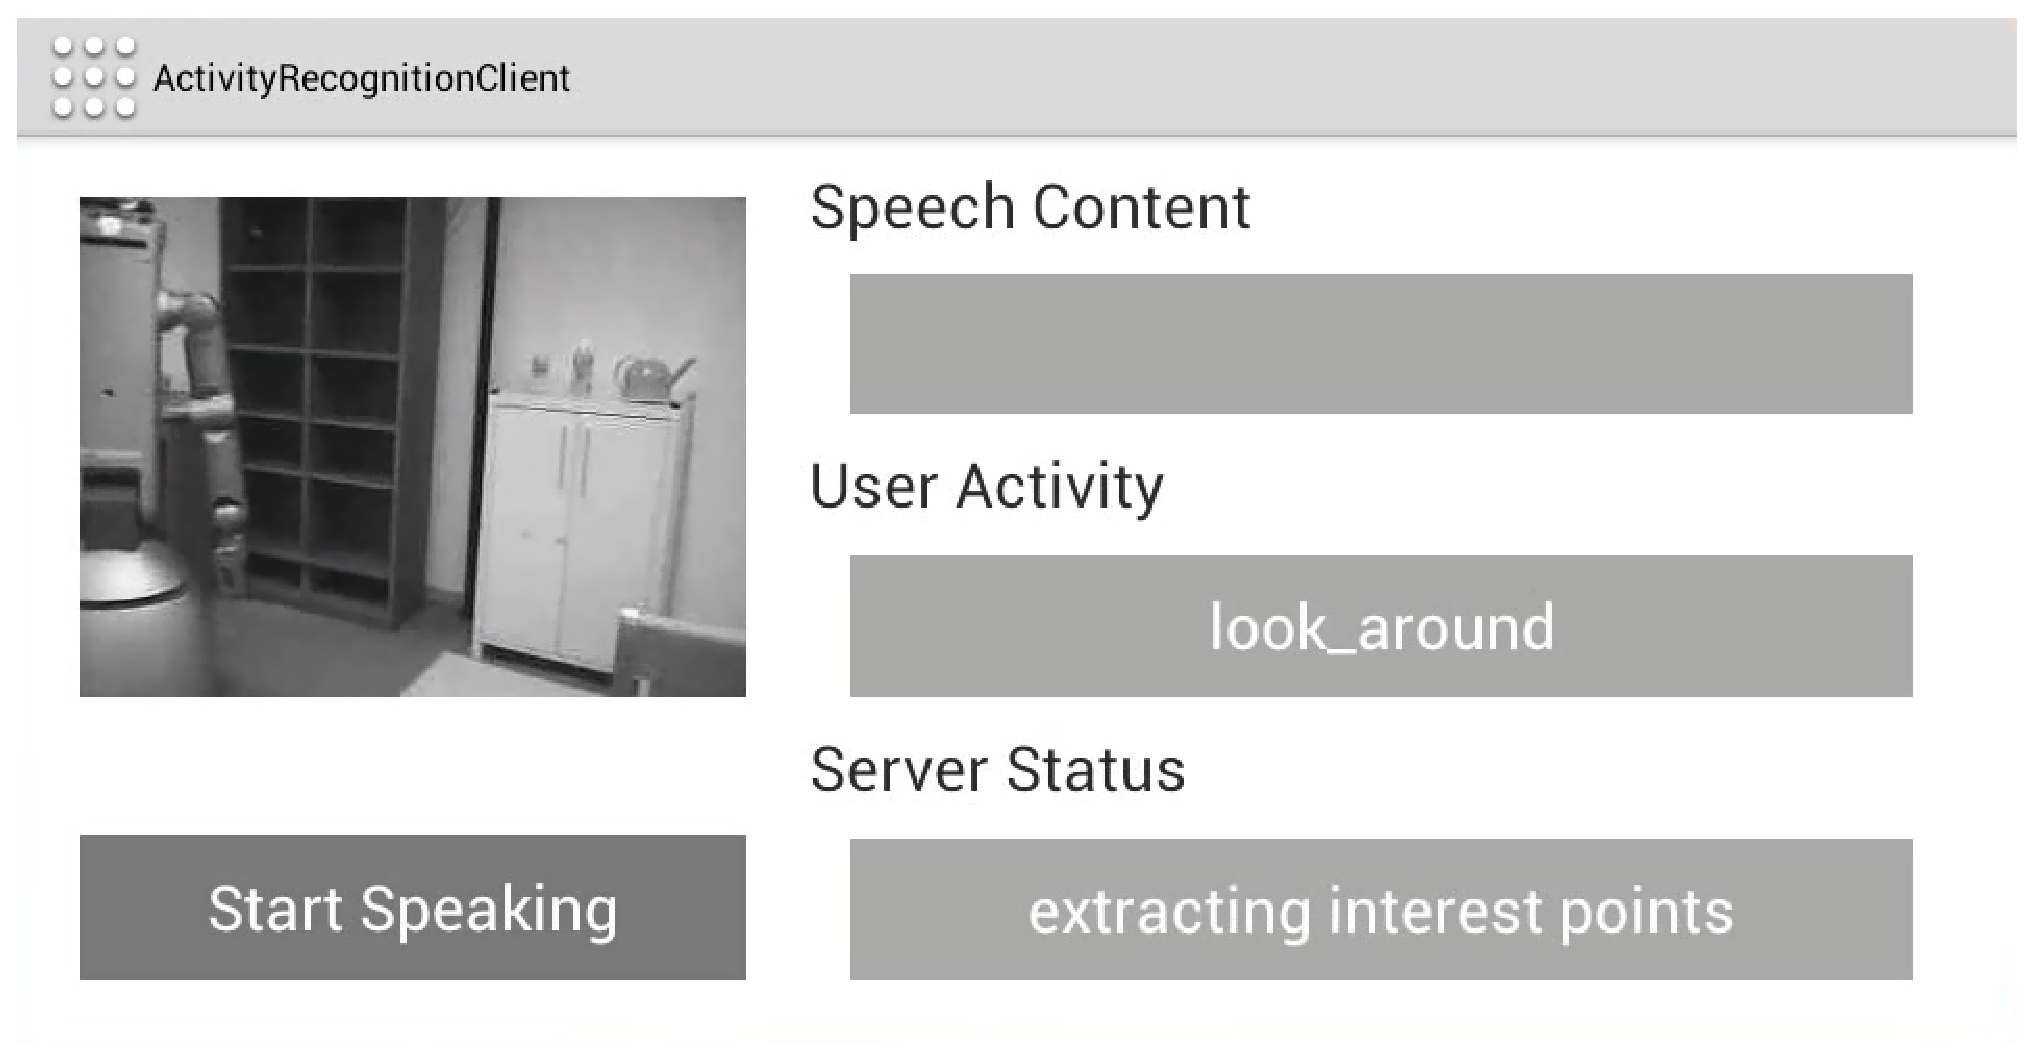
\includegraphics[width=75mm]{figure/experiment_2_proactive_2_a.eps}
    \end{center}
  \end{minipage}
%
\end{tabular}
\caption{辺りを見回している場合}
\label{fig:experiment_2_proactive_2}
\end{figure}

以上のように,両者の行動は正しく認識され,サービスロボットから能動的なサービスの開始を行うことが出来た.